\chapter{Electronique}

\newpage

\section{Puissance consommée par un AO $\bullet\circ\circ\circ$}
 
On souhaite alimenter un dispositif électrique (en rouge) modélisé par une résistance de charge $R_c$ avec une tension nominale $V_{nom}$. On dispose pour cela d'une source de tension (en bleue) mais dont la tension de sortie maximale $V_{max}$ est $V_{max} = V_{nom}/2$, insuffisante pour l'usage voulu. On introduit un montage intermédiaire pour compenser l'insuffisance de la source. 

\begin{figure}[!h]
\centering
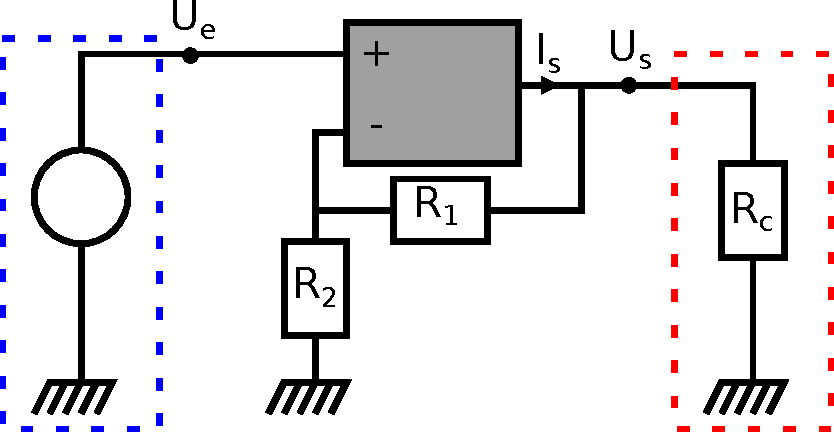
\includegraphics[width=0.5\linewidth]{electronique_puissance_AO.pdf}
\end{figure}

\begin{enumerate}
	\item Calculer $U_s$ en fonction de $U_e$ et déterminer le rôle de ce montage. Comment doit-on choisir $R_1$ et $R_2$ pour que $U_s = V_{nom}=2V_{max}$ ?
	\item On suppose dans un premier temps que $R_c=\infty$, cad que la résistance de charge n'est pas connectée au circuit. Quelle est la puissance électrique émise par l'AO ?
	\item On suppose maintenant que le circuit est connecté à la charge, cad que $R_c$ est finie. Quelle est désormais la puissance dégagée par l'AO ?
	\item Comment choisir $R_1$ et $R_2$ de sorte à minimiser la puissance sortie par l'AO ?
\end{enumerate}

\newpage

\begin{correction}

\begin{enumerate}
	\item Amplificateur non-inverseur $u_s = \frac{R_1+R_2}{R_2}u_e$. Pour que $U_s = V_{nom}=2V_{max}$ il faut que le montage double la tension, cad $R_1=R_2$.
	\item  Si $R_c=\infty$, alors le courant dans la charge $i_c$ est nul. Alors $P=u_si_s= \frac{R_1+R_2}{R_2^2}u_e^2$. L'AO consomme de l'énergie même s'il n'y a aucune puissance délivrée à la charge !
	\item Soit $i_1$ le courant traversant $R_1$ et $R_2$. Alors la loi des nœuds donne : $i_s-i_1-ic=0$ (signe pris tq les puissances soient positives). On a alors :
	\begin{equation}
		P=u_si_s=\frac{R_1+R_2}{R_2^2}u_e^2+\frac{(R_1+R_2)^2}{R_2^2R_c}u_e^2
	\end{equation}
	\item On prend $R_2\gg R_c$, le premier terme de dissipation de l'AO devient négligeable devant la puissance envoyée à la charge.
\end{enumerate}

\end{correction}

\newpage

\section{Montage passe-bas $\bullet\bullet\circ\circ$}

On considère le montage suivant. L'ALI est supposé idéal.

\begin{figure}[!h]
\centering
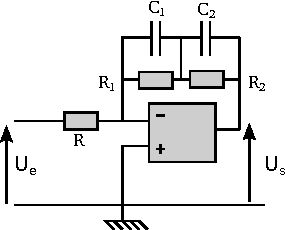
\includegraphics[width=0.5\linewidth]{electronique_circuit_6.pdf}
\end{figure}

\begin{enumerate}

	\item Montrer que la fonction de transfert de ce filtre s'écrit sous la forme :
\begin{equation}
	H=H_0\frac{1+j\omega/\omega_0}{(1+j\omega/\omega_1)(1+j\omega/\omega_2)}
\end{equation}
On donnera l'expression de $\omega_0$, $\omega_1$ et $\omega_2$.

\item Tracer le diagramme de Bode correspondant en fonction des différentes pulsations en jeu. Expliciter les cas possibles.

\item On considère désormais que $R=R_1=R_2$ et $C_1=C_2=C$. Simplifier la fonction de transfert, en introduisant $\omega_0=1/RC$. A quel type de filtre à t-on affaire ?

\item On envoie en entrée le signal suivant :
\begin{equation}
	U_e(t) = \frac{4U_0}{\pi}\sum_{p=0}^{\infty}\frac{1}{2p+1}\sin(2(p+1)\omega t)
\end{equation}
On suppose que $\omega\gg\omega_0$. Quel est le signal de sortie $U_s$ ? Donner son allure et commenter. 

\end{enumerate}

\newpage

\begin{correction}

\begin{enumerate}

	\item Fonction de transfert :
\begin{equation}
	H=\frac{u_s}{u_e}=\frac{R_1+R_2}{R}\frac{1+j\frac{R_1R_2}{R_1+R_2}(C_1+C_2)\omega}{(1+jR_1C_1\omega)(1+jR_2C_2\omega)}=H_0\frac{1+j\omega/\omega_0}{(1+j\omega/\omega_1)(1+j\omega/\omega_2)}
\end{equation}
donc $H_0=\frac{R_1+R_2}{R}$, $\omega_0=\frac{R_1+R_2}{R_1R_2(C_1+C_2)}$, $\omega_1=1/R_1C_1$ et $\omega_2=1/R_2C_2$

	\item Diagramme de Bode : on décompose en somme des diagrammes de Bode des différents produits.

\textbf{Cas $\omega_0<\omega_1<\omega_2$ :}
\centering
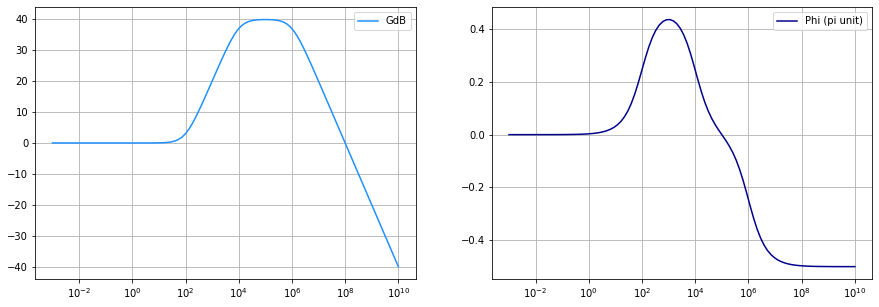
\includegraphics[width=0.8\linewidth]{electronique_exo2_0.png}

\textbf{Cas $\omega_1<\omega_0<\omega_2$ :}
	\centering
	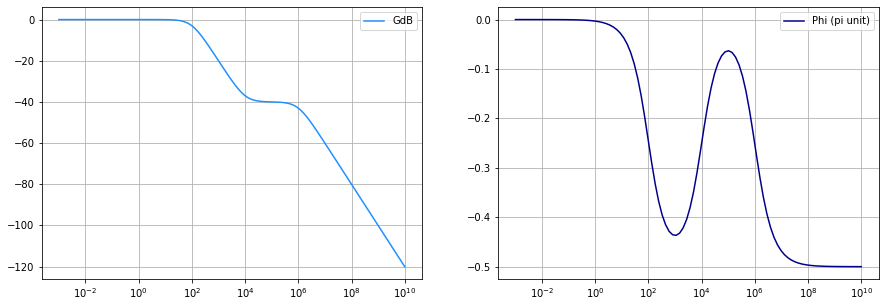
\includegraphics[width=0.8\linewidth]{electronique_exo2_1.png}

\textbf{Cas $\omega_1<\omega_2<\omega_0$ :}
	\centering
	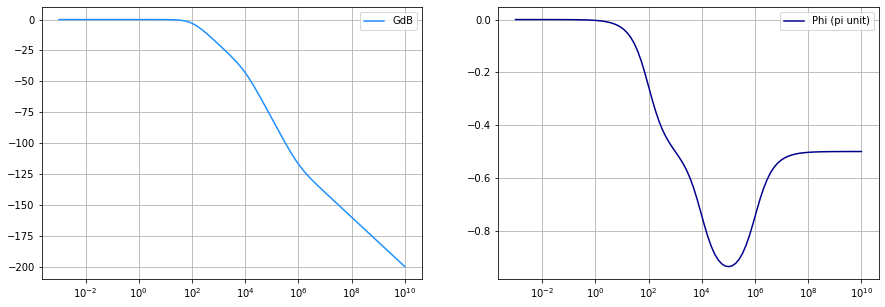
\includegraphics[width=0.8\linewidth]{electronique_exo2_2.png}

	\item Comme $\omega_0=\omega_1=\omega_2$ et $H_0=2$, la fonction de transfert se simplifie en : 
\begin{equation}
	H=\frac{2}{(1+j\omega/\omega_0)}
\end{equation}	
C'est un filtre passe-bas d'ordre 1.

\item Le signal d'entrée est un signal créneau (pair, avec les cosinus) : on reconnait la décroissance typique en $1/n$ avec les $n$ impairs seulement. Les coefficients de Fourier sont :

\begin{equation}
	\left\lbrace
	\begin{array}{lll}
		C_n &= \frac{4U_0}{\pi}\frac{1}{2(p+1)}\\
		\varphi_n &= -\frac{\pi}{2} \\
	\end{array}\right.
\end{equation}

On rappelle l'écriture de la décomposition de Fourier :
\begin{equation}
	U_e(t) = \sum_{p=0}^{\infty}C_n\cos(n\omega t+\varphi_n)
\end{equation}

La fonction de transfert, dans le cas où $\omega\gg\omega_0$, peut se simplifier en $H\simeq\frac{2\omega_0}{j\omega}$. Les coefficients de Fourier du signal de sortie sont alors : 

\begin{equation}
	\left\lbrace
	\begin{array}{lll}
		C'_n & = \frac{4U_0}{\pi}\frac{1}{2(p+1)}\times |H(2(p+1)\omega)|\\

		\varphi_n' &= -\frac{\pi}{2}+\mathbf{arg}\left(\frac{2\omega_0}{j\omega} \right)  \\
	\end{array}\right.
\end{equation}

On obtient donc :
\begin{equation}
	\left\lbrace
	\begin{array}{lll}
		C'_n & = \frac{4U_0}{\pi}\frac{2}{(2(p+1))^2}\frac{\omega_0}{\omega}\\
		\varphi_n' &= -\frac{\pi}{2}-\frac{\pi}{2} \\
	\end{array}\right.
\end{equation}

Le signal de sortie est donc :

\begin{equation}
	U_s(t) = \frac{2U_0}{\pi}\sum_{p=0}^{\infty}\frac{1}{(2p+1)^2}\cos(2(p+1)\omega t -\pi)
\end{equation}

On reconnait la décroissance en $1/n^2$ typique d'un signal triangulaire. C'est normal : le filtre se comporte ici comme un intégrateur.

\end{enumerate}

\end{correction}

\newpage

\section{Filtre passif $\bullet\bullet\bullet\bullet$}

On considère le filtre suivant :

\begin{figure}[!h]
\centering
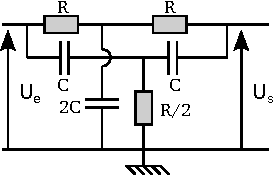
\includegraphics[width=0.5\linewidth]{electronique_circuit_2.pdf}
\end{figure}

\begin{enumerate}

	\item[$\spadesuit$] Quel est le comportement de ce filtre à basse et haute fréquence ? 
	
	\item[$\spadesuit$] Montrer que la fonction de transfert peut s'écrire sous la forme :
	\begin{equation}
		H(x) =\frac{1+(jx)^2}{1+4jx + (jx)^2}
	\end{equation}
	où $x=\omega/\omega_0$ avec $\omega_0$ une pulsation que l'on déterminera. Tracer le diagramme de Bode correspondant. 
	
	\item[$\spadesuit$] Déterminer la bande "coupante" $\Delta\omega$, cad la plage de pulsations $\Delta\omega$ pour lesquelles $G^{dB}(\omega)\leq G^{dB}_{max} - 3$. On rappelle que $20\log\left( \sqrt{2}\right)\simeq3 $.
	
	\item[$\spadesuit$] On envoie le signal $U_e(t)=U_0\cos^3(\omega t)$ en entrée, avec $\omega=\omega_0/3$. Déterminer le signal de sortie $U_s(t)$. Tracer schématiquement les signaux.

\end{enumerate}

\newpage

\begin{correction}

Le courant de sortie est supposé nul.

\begin{enumerate}
	\item Comportement : BF, $u_e=u_s$ et HF, $u_e=u_s$, c'est un filtre coupe-bande (l'inverse d'un passe-bande, qui ne laisse rien passer à BF et HF). En BF, le circuit est "flottant", cad il n'es tplus connecté à la masse. Comme l'intensité de sortie est considérée comme nulle, la chute de tension aux bornes des résistances est nulle.
	
	\item
		Pour la fonction de transfert, on fait une loi des nœuds en A (entre les 2 résistances du haut), en B (entre les 2 capa du milieu) et à la sortie :
		
\begin{equation}
	\left\lbrace
	\begin{array}{lll}
		 \frac{u_e-u_A}{R} + \frac{u_s-u_A}{R} -2jC\omega u_A = 0\\
		 \\
		 jC\omega(u_e-u_B) +  jC\omega(u_s-u_B) - \frac{2}{R}u_B =0  \\
		 \\
		 \frac{u_A-u_s}{R} + jC\omega(u_B-u_s)=0
	\end{array}\right.
\end{equation}

Avec les deux premières lignes, on trouve :

\begin{equation}
	\left\lbrace
	\begin{array}{lll}
		 u_A = \frac{u_e+u_s}{2(1+jRC\omega)}\\
		 \\
		 u_B = \frac{u_e+u_s}{2(1+1/jRC\omega)} \\
	\end{array}\right.
\end{equation}

	On trouve alors en réinjectant dans la dernière équation :
	\begin{equation}
		H =\frac{1+(jRC\omega)^2}{1+4jRC\omega + (jRC\omega)^2}
	\end{equation}
	
	Diagramme de Bode :
Diagramme assymptotique :  $\forall \omega, H=0$ et pour $\omega=\omega_0=1/RC$, dirac à "l'envers" avec $H=-\infty$. C'est bien un coupe-bande.
	\centering
	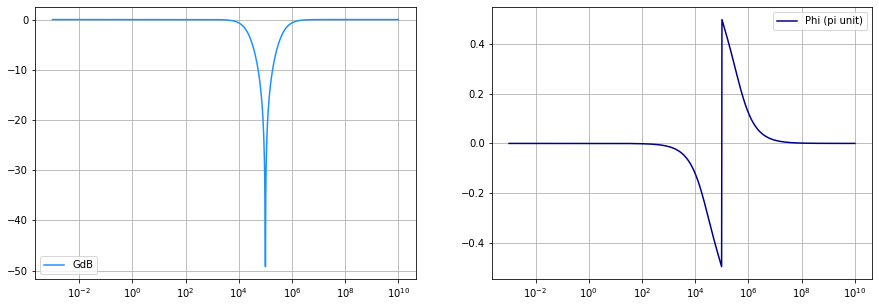
\includegraphics[width=0.8\linewidth]{electronique_exo3_0.png}

	\item Pour la bande-coupante, on cherche les $\omega$ de telle sorte que :
\begin{equation}
	G_{DB} = -20\log \left( \frac{|1-x^2|}{\sqrt{(1-x^2)^2+16x^2}}\right) = -20\log\left(\frac{1}{\sqrt{2}} \right) \simeq 3
\end{equation}	
	en posant $x=RC\omega$.
On tombe alors sur l'équation $(1-x^2)^2=16x^2$, et en enlevant le carré :
\begin{equation}
	x^2\pm 4x -1 =0
\end{equation}
Avec le signe $\pm$, il y a 4 solutions possibles (2 par équations, qui ont 2 solutions chacunes). Les seules solutions positives sont $\omega_{\pm}=\frac{\pm 2+\sqrt{5}}{RC}$.

	\item On peut montrer facilement que le signal d'entrée peut s'écrire sous la forme :
	\begin{equation}
		U_e(t)=\frac{1}{4}\left( 3\cos(\omega t) + \cos(3\omega t)\right) 
	\end{equation}
	
	On a donc deux harmoniques, à $\omega$ et $3\omega$, soit :

\begin{equation}
	\left\lbrace
	\begin{array}{lll}
		C_1 & = \frac{3}{4}, \quad \varphi_1=0 \\

		C_3 & = \frac{1}{4}, \quad \varphi_3=0  \\
	\end{array}\right.
\end{equation}	

Ces harmoniques deviennent après sortie du filtre : 
\begin{equation}
	\left\lbrace
	\begin{array}{lll}
		C_1 & = \frac{3}{4}\times |H(\omega)|, \quad \varphi_1=0 + \mathbf{arg}\left(H(\omega) \right)  \\

		C_3 & = \frac{1}{4}\times |H(3\omega)|, \quad \varphi_3=0 + \mathbf{arg}\left(H(3\omega) \right)  \\
	\end{array}\right.
\end{equation}		

Comme $|H(3\omega)| = |H(\omega_0)| = 0$, l'harmonique 3 n'a aucune contribution. Dès lors, pur la première harmonique $x=\omega/\omega_0=1/3$ : 
\begin{equation}
	\left\lbrace
	\begin{array}{lll}
		C_1 & = \frac{3}{4}\times \left|\frac{1-\frac{1}{9}}{1+j\frac{4}{3}-\frac{1}{9}} \right| =\frac{4}{\sqrt{52}} \simeq\frac{1}{2} \\

		\varphi_1 & = -\mathbf{arg}\left( 1+j\frac{4}{3}-\frac{1}{9}\right) =\arctan\left( \frac{27}{32}\right) \simeq \frac{\pi}{4} \\
	\end{array}\right.
\end{equation}		
	
En très grosse approximation, on peut donc dire que :
\begin{equation}
	U_s(t) \simeq \frac{1}{2}\cos(\omega t + \pi/4)
\end{equation}	

\centering
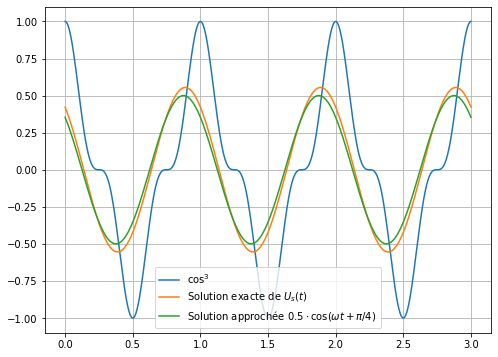
\includegraphics[width=0.5\linewidth]{electronique_exo3_1.png}
	
\end{enumerate}

\end{correction}

\newpage

\section{Filtre avec ALI $\bullet\bullet\circ$}

Dans tout l'exercice, les ALI seront supposés idéaux.

\begin{enumerate}

\item Explicitez la fonction de transfert de ce filtre, puis calculez son gain et sa phase. On notera $\omega_0$ sa pulsation caractéristique. Quel est son rôle ?
\begin{figure}[!h]
\centering
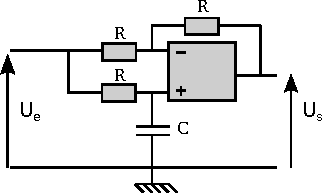
\includegraphics[width=0.5\linewidth]{electronique_circuit_.pdf}
\end{figure}

\item On exprime le signal d'entrée $U_e$ par sa transformée de Fourier :
\begin{equation}
U_e(t) = \sum_n C_n\cos(n\omega t + \varphi_n)
\end{equation}
Déterminer l'expression du signal $U_s$ de sortie sous la forme d'une transformée de Fourier, en fonction des coefficients $C_n$ et des caractéristiques du circuit.

\item
Pour quelles conditions sur le circuit et le signal d'entrée trouve t-on que le circuit retarde un signal périodique sans le déformer, c'est-à-dire que $U_{s}(t)=U_{e}(t-\tau)$ ? Exprimez alors ce retard $\tau$ en fonction de $R$ et $C$.

\item On envoie en entrée le signal suivant :
\begin{equation}
U_{e}(t) = U_{0}\cos^{3}(\omega t)
\end{equation}

Décrire l'effet du filtre sur ce signal pour $\omega = \frac{\omega_{0}}{3}$ et $\omega=10^{-2}\omega_0$, et donner l'allure du signal de sortie. On donne $\arctan(1/3)\simeq\pi/10$.

\item
On suppose le condensateur déchargé à $t=0$. On envoie un échelon de tension $E$ en entrée. Quelle est la sortie ? Commenter.
\end{enumerate}

\newpage

\begin{correction}

\begin{enumerate}
	\item
	$H=\frac{1-jRC\omega}{1+jRC\omega}$. On remarque que $\mid H\mid=1$, mais que $\varphi=-2\arctan(RC\omega)=-2\arctan(\omega/\omega_0)$, avec $\omega_0=1/RC$. On peut écrire alors $H$ sous la forme :
	\begin{equation}
		H=e^{-2j\arctan(RC\omega)}
	\end{equation}
C'est un filtre déphaseur.

	\item
	On part de la décomposition de Fourier d'un signal (quelconque) d'entrée :
\begin{equation}
	U_e(t) = \sum_n C_n\cos(n\omega t + \varphi_n)
\end{equation}	
Après le passage dans le filtre, le signal de sortie :	
\begin{equation}
	\begin{array}{lll}
		U_s(t) & = \sum_n C_n|H(n\omega)|\cos(n\omega t + \varphi_n + \mathbf{arg}(H(n\omega)) \\

		 & = \sum_n C_n\cos(n\omega t + \varphi_n -2\arctan(RCn\omega)) \\
	\end{array}
\end{equation}	

		
	\item pour obtenir une forme retardée comme proposée dans l'énoncé, il faut factoriser par le $n\omega$ compris dans le $\arctan$. On le linéarise dans le cas où $RCn\omega\ll1$, cad $\omega\ll\omega_0$ avec $1/\tau=1/2RC$. 
	
	Dans ce cas-là :
\begin{equation}
	\begin{array}{lll}
		U_s(t) & = \sum_n C_n\cos(n\omega t + \varphi_n -2RCn\omega) \\

		 & = \sum_n C_n\cos(n\omega (t-\tau) + \varphi_n) \\
		 &= U_e(t-\tau)
	\end{array}
\end{equation}			
	Il faut donc que $\omega\ll 1/RC$, avec toutes les harmoniques qui valident cette condition (ex : signal triangulaire, avec une décroissance rapide de l'amplitude des harmoniques).
	
	\item On décompose le signal en une série de cosinus : $\cos^3(\omega t)=\frac{1}{4}(3\cos(\omega t) + \cos(3\omega t))$.
	Le signal de sortie sera donc : 
	\begin{equation}
	U_s(t) = \frac{1}{4}\left[ 3\cos(\omega t - 2\arctan(\omega/\omega_0)) + \cos(3\omega t - 2\arctan(3\omega/\omega_0))\right] 
	\end{equation}
	Pour $\omega = \frac{\omega_{0}}{3}$, on a :
\begin{equation}
	\begin{array}{lll}
		U_s(t) & = \frac{3}{4}\cos(\omega t - 2\arctan(1/3)) + \frac{1}{3}\cos(3\omega t - 2\arctan(1) \\

		 & \simeq \frac{3}{4}\cos(\omega t - \pi/5) + \frac{1}{3}\cos(3\omega t - \pi/2)\\
	\end{array}
\end{equation}		
	Pour $\omega = 10^{-2}\omega_0$, on a la condition $\omega\ll\omega_0$, avec un retard de phase $\varphi = 2\cdot10^{-2}$.
	
	\item Pour $t<0$, le condensateur est déchargé donc $u_e(t)=u_s(t)=0$. Pour $t\geq0$, le condensateur se charge donc $u_-(t) = E(1-e^{-t/RC})$, et alors :
	\begin{equation}
		u_s(t)=2E(1-e^{-t/RC}) - E
	\end{equation}
	Le signal finit bien par "redevenir" celui d'entrée (car $H=1$) mais un retard. Attention, ici c'est une transformation de Fourier et non une série de Fourier qu'il faut opérer. 
	
\end{enumerate}

\end{correction}

\newpage

\section{Etude de deux bobines d'électroaimant}

On considère un électroaimant constitué de deux bobines $L_1$ et $L_2$, couplées selon la relation $L_1=L_e+\delta L$ et $L_2=L_e-\delta L$, avec $\delta L\ll L_e$. L'électroaimant, alimenté par une tension $e(t)=E\cos(\omega t)$, peut être modélisé comme une résistance $R$ en série avec les deux bobines : 

\begin{figure}[!h]
\centering
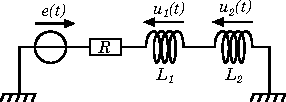
\includegraphics[width=0.6\linewidth]{electronique_soustracteur1.pdf}
\end{figure}

\begin{enumerate}

\item Pour pour connaitre la position de l'électroaimant, on souhaite connaitre $\delta L$ en utilisant les tensions $u_1$ et $u_2$ aux bornes des bobines $L_1$ et $L_2$. 

Déterminer les tensions $u_1$ et $u_2$ en fonction de $e(t)$, $R$, $L_1$ et $L_2$.

\item Pour accéder à $\delta L$, on utilise le montage soustracteur suivant :

\begin{figure}[!h]
\centering
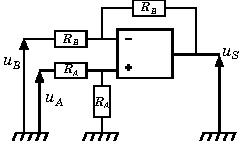
\includegraphics[width=0.6\linewidth]{electronique_soustracteur2.pdf}
\end{figure}

\begin{enumerate}

 \item Déterminer la tension $u_s$ de sortie en fonction de $u_A$ et $u_B$ et montrer qu'il s'agit d'un montage soustracteur.
 
 \item Comment relier le montage soustracteur à l'électroaimant de sorte à avoir $u_s=u_1-u_2$ (c'est-à-dire $u_A=u_1$ et $u_B=u_2$) ? Préciser comment choisir les résistances $R_A$ et $R_B$.
 
 \item On suppose que le montage précédent est réalisé, c'est-à-dire que $u_s=u_1-u_2$. Exprimer alors la fonction de transfert $H$ de l'ensemble sous la forme :
 \begin{align*}
 H(\omega)=\frac{u_s}{e}=H_0\frac{j\omega/\omega_0}{1+j\omega/\omega_0}
\end{align*}  
où $\omega_0$ et $H_0$ sont des fonctions de $L_e$, $R$ et $\delta \omega$.	

\item Tracer le diagramme de Bode de $H(\omega)$. Dequel type de filtre s'agit-il ? Dans quel gamme de fréquence doit-on se placer pour avoir une sorte indépendante de la fréquence et proportionnel à $\delta L$ ?

\end{enumerate}

\end{enumerate}

\newpage

\begin{correction}

\begin{enumerate}

\item On commence par $u_2$, qui est le plus simple à calculer (pont-diviseur) :
\begin{align*}
	u_2=\frac{jL_2\omega}{j(L_1+L_2)\omega + R}e
\end{align*}
Pour $u_1$, il faut tenir compte qu'il s'agit de la tension aux bornes de la bobines (et non par rapport à la masse). Le pont diviseur donne donc :
\begin{align*}
	u_1&=\frac{jL_1\omega}{jL_1\omega+R}(e-u_2) \\
	&=\frac{jL_1\omega}{jL_1\omega+R}\times\frac{jL_1\omega+R}{j(L_1+L_2)\omega + R}e\\
	&=\frac{jL_1\omega}{j(L_1+L_2)\omega + R}e
\end{align*}
\item

\begin{enumerate}

 \item Une loi des noeuds à l'entrée $+$ donne : $u_A=2u_+$, à l'entrée $-$ : $u_s+u_B=2u_-$. On a donc $u_s=u_1-u_2$.
 
 \item Il faut prendre au garde que les tensions $u_1$ et $u_2$ sont prises aux bornes des bobines et non par rapport à la masse, contrairement aux tensions du soustracteur. Il faut réaliser le montage suivant pour avoir la tension $u_1-u_2$ à la sortie du montage :
 
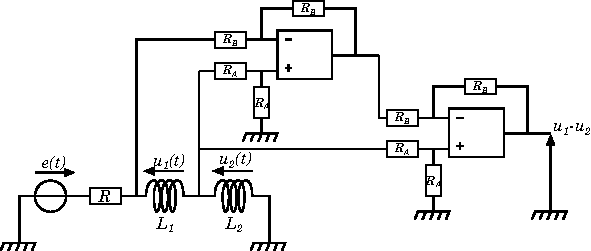
\includegraphics[width=0.9\linewidth]{electronique_soustracteur3.pdf}

D'autre part, pour éviter que la mesure des tensions ne perturbe le circuit de l'électroaimant, on prend les résistances $R_A$ et $R_B$ très grades devant $R$, $L_1\omega$ et $L_2\omega$.
 
 \item On a :
 \begin{align*}
 	H(\omega)=&\frac{u_1-u_2}{e} \\
 	=&\frac{j(L_1-L_2)\omega}{j(L_1+L_2)\omega+R}\\
 	=&\frac{L_1-L_2}{L_1+L_2}\frac{j\omega(L_1+L_2)/R}{1+j\omega(L_1+L_2)/R}
 \end{align*}
 On a donc $\omega_0=(L_1+L_2)/R=2L_e/R$ et $H_0=(L_1-L_2)/(L_1+L_2)=\delta L/L_e$.

\item Filtre passe-haut (cf diagramme de Bode du cours). On doit se placer dans une gamme de fréquence $\omega\gg\omega_0$, à ce moment là $H\simeq \delta L/L_e$.

\end{enumerate}

\end{enumerate}

\end{correction}